\documentclass[12pt,a4paper]{article}
\usepackage[italian]{babel}
\usepackage[T1]{fontenc}
\usepackage[latin1]{inputenc}
\usepackage{graphicx}
\usepackage{amsmath}
\usepackage{subfig}
\usepackage[a4paper,top=1.5cm,bottom=1.4cm,left=1.4cm,right=1.4cm]{geometry}
\date{}
\begin{document}
\title{Ipersonica\\ Esercitazione 4 \\ Prof.re Renato Paciorri}
\author{Matteo Hakimi 1455230}
\maketitle
\begin{figure}[htbp]
\centering

\includegraphics[width=100mm]{Immagini/1}
\end{figure}
\newpage
\tableofcontents
\newpage
\section{Introduzione}
Si vuole studiare il flusso di una miscela reagente in campo ipersonico. In particolare nella prima sezione, verr� studiata l'evoluzione temporale della reazione di dissociazione dell'azoto molecolare al variare delle variabili di stato: temperatura e pressione; enfatizzando i tempi di reazione nonch� il valore del grado di dissociazione all'equilibrio al variare di dette grandezze.\\
Si proceder� con lo studio dell'evoluzione del flusso unidimensionale stazionario a valle di urto normale, mettendo in evidenza le differenze che si manifestano tra flusso reagente e non.\\
Successivamente, verr� analizzato il caso di un flusso reagente stazionario in un condotto convergente divergente, considerando note le condizioni di flusso nella sezione di gola .\\
\section{Cinetica di dissociazione}
In questa sezione ci dedicheremo allo studio di evoluzione temporale di una miscela composta da azoto molecolare $N_{2}$ e atomico $N$ avendo fissanto le condizioni di temperatura e pressione di reazione.\\
Bisogna notare come la reazione di dissociazione dell'azoto sia una reazione endotermica, per cui aver assunto che questa avvenga a temperatura costante significa fornire in ogni istante la quantit� di calore $\Delta Q$ sottratta dalla reazione stessa.
Effettuando un confronto col grado di dissociazione all'equilibrio ottenuto analiticamente.
Successivamente il calcolo verr� reiterato cambiando le varibili di stato T e p.\\
Le reazioni di dissociazione che consideremo sono:\\
$$N_{2}+N_{2}\rightleftharpoons2N+N_{2}$$ 
$$N_{2}+N\rightleftharpoons3N$$\\\\
L'equazione di conservazione della specie nel caso dell'azoto molecolare diventa
$$\frac{d[N]}{dt}=2{k_{f}[N_{2}]^2-2k_{b}[N]^2[N_{2}]}+2{k_{f}[N][N_{2}]-2k_{b}[N]^3}$$\\\\
Avendo indicato con $k_{f}$ la costante di velocit� di reazione diretta ({\itshape{forward}}) e con $k_{b}$ quella inversa ({\itshape{backward}}).
In particolare: 
$$k_{f}=C_{f}T^{\alpha}e^{\frac{-Td}{T}}$$ 
$$k_{b}=\frac{k_{f}}{k_{c}}$$\\\\
dove $\alpha$ � un esponente caratteristico della reazione presa in considerazione, e $C_{f}$ una costante moltiplicativa, in paricolare $\alpha=-1.6$ e $C_{f}=7\cdot10^{15}$ $\frac{m}{mol\cdot s}$\\
Indicando con $\rho$ la densit� e con $\alpha$ il grado di dissociazione, e considerando l'equazione di stato:\\\\
$$\rho=\frac{p}{R_{mix}T}=\frac{2pM_{N}}{(1+\alpha)R_{0}T}$$\\\\
dove con $R_{0}$ si � indicata la costante universale dei gas, $R_{0}=8.314$ $[JK^{-1}mol^{-1}]$, e sapendo che $[N]=\frac{\rho\alpha}{PM_{N}}$ e che $[N_{2}]=\frac{\rho(1-\alpha)}{2PM_{N}}$ , l'equazione di conservazione della specie, diventa:\\
\begin{equation}
	\frac{d\alpha}{dt}=\frac{\dot{w}_{\alpha}}{\rho}
\end{equation}
avendo indicato con $\dot{w}_{\alpha}$ il termine reagente e pari a:\\
\begin{equation}
	\dot{w}_{\alpha}=\rho(1+\alpha)^2\left[k_{f}(T)\frac{(1-\alpha)p}{(1+\alpha)R_{0}T}-4k_{b}(T)\left(\frac{\alpha p}{(1+\alpha)R_{0}T}\right)^2\right]
\end{equation}
Mentre per quanto riguarda il valore del grado di dissociazione all'equilibrio, ponendo $\frac{d[N]}{dt}=0$ si ricava:\\
$$\alpha_{eq}=\sqrt{\frac{k_{c}R_{0}T}{4p+k_{c}R_{0}T}}$$
la costante di equilibrio $k_{c}$ nel caso di reazione di dissociazione dell' azoto � pari a:\\
\begin{equation}
	k_{c}(T)=a_{1}e^{a_{2}+a_{3}zp+a_{4}zp^2+a_{5}zp^3+a_{6}zp^4}
\end{equation}
dove $zp=10^4/T$ e i coefficienti $a_{i}$, $  i=1,..,6$, sono ricavati sperimentalmente.\\
In particolare per la reazione di dissociazione/ricombinazione dell'azoto si ha:\\
$$a_{1}=10^6 mol/m^3\quad
a_{2}=3.898\quad
a_{3}=-12.661\quad
a_{4}=0.683\quad
a_{5}=-0.118\quad
a_{6}=0.006$$
Viene implementato su codice Matlab l'equazione differenziale sostituendo la (2) nella (1) e tenendo conto della (3).
Vengono riportati in figura i risultati ottenuti, nel caso di pressione costante al variare della temperatura di reazione, e viceversa.\\
\newpage
\begin{figure}[htbp]
	\centering
	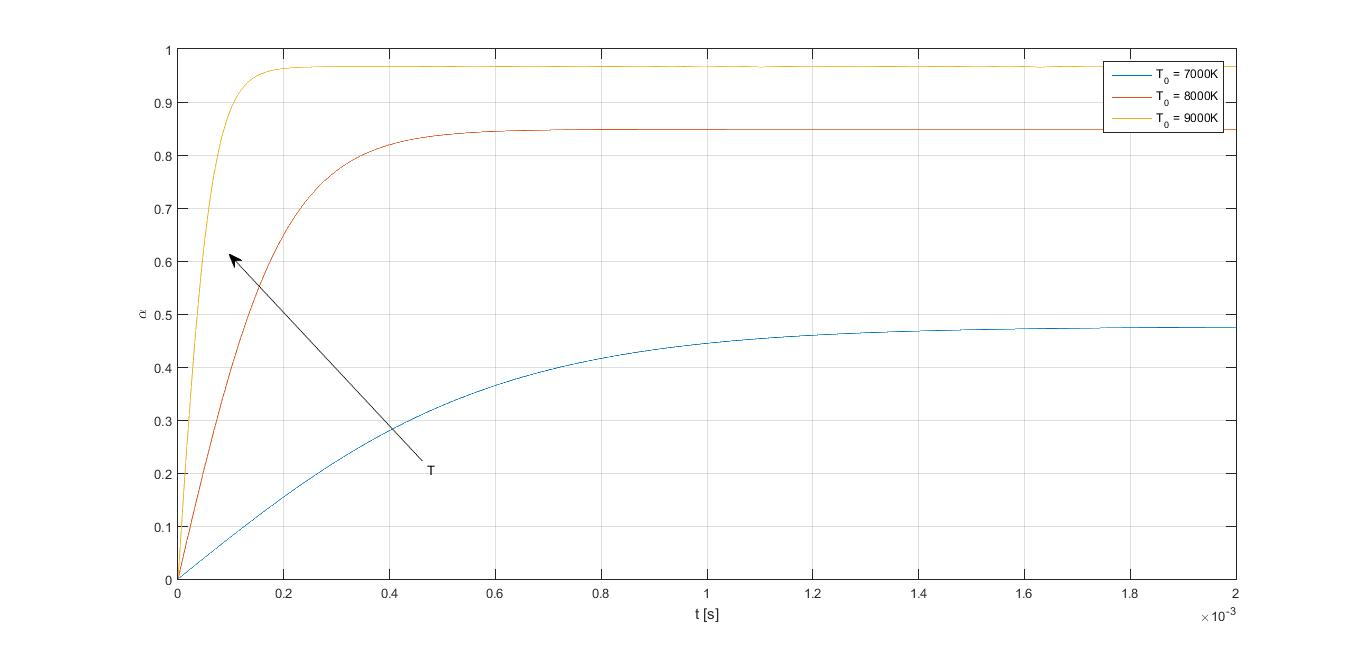
\includegraphics[width=150mm]{Immagini/alpha_T}
	\caption{Andamento del grado di dissociazione  funzione del tempo, al variare della temperatura }
\end{figure}
\begin{figure}[htbp]
	\centering
	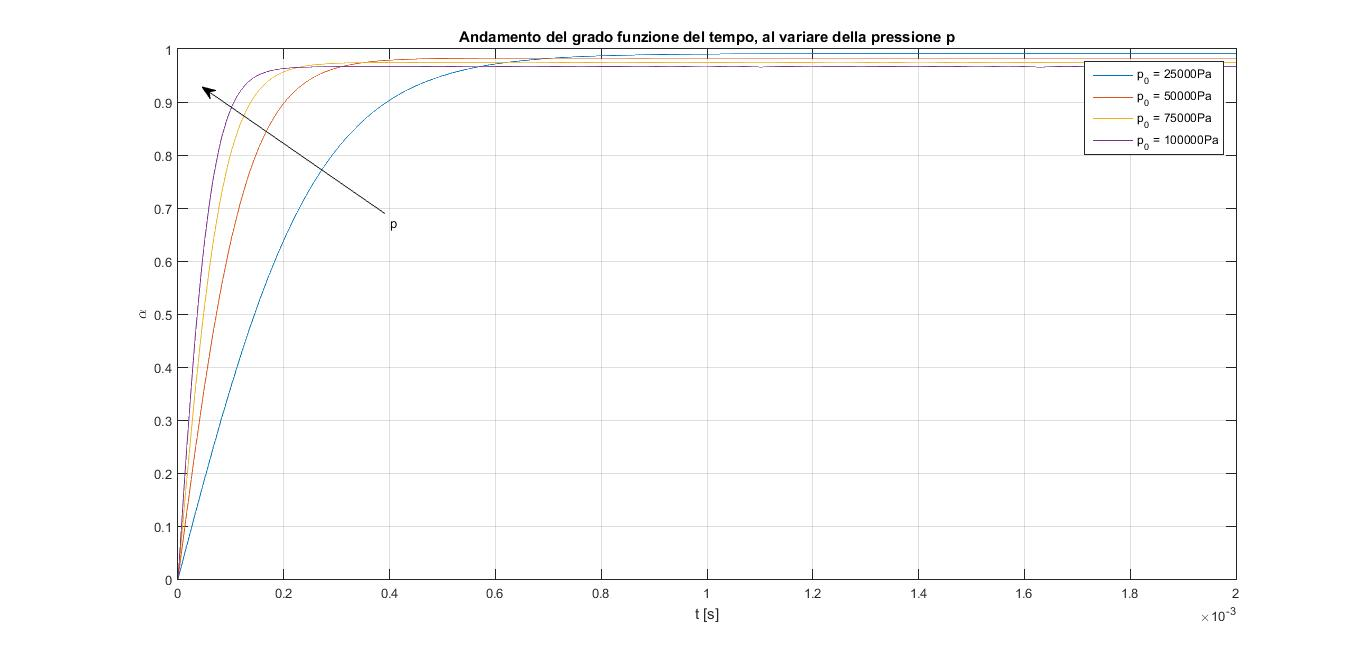
\includegraphics[width=150mm]{Immagini/alpha_p}
	\caption{Andamento del grado di dissociazione  funzione del tempo, al variare della pressione }
\end{figure}

Si nota come in entrambi i casi i tempi di reazione siano estremamente brevi.
Si nota inoltre come all'aumentare della temperatura il grado di dissociazione all'equilibrio risulta pi� elevato.
\section{Flusso reagente a valle dell' urto normale}
In questa sezione si vuole studiare il flusso di un gas formato da  azoto molecolare, in campo ipersonico, che attraversa un urto normale.  Il modello adottato � quello di flusso reagente (dissociazione/ricombinazione) non viscoso unidimensionale stazionario.\\
Inoltre poich� lo spessore dell'urto � dell'ordine di $10$ cammini medi possiamo assumere per semplicit� il modello di {\itshape urto parzialmente disperso}, intendendo che il gas non subisce nessuna reazione chimica nell'urto stesso.\\
\newpage
In particolare per una miscela binaria possiamo scrivere:\\

\begin{equation}
	u\frac{d\rho}{dx}+\rho\frac{du}{dx}=0\\
\end{equation}
\begin{equation}
	u\frac{du}{dx}+\frac{1}{\rho}\frac{dp}{dx}=0\\
\end{equation}
\begin{equation}	
	u\frac{dH}{dx}=0\\
\end{equation}
\begin{equation}	
	u\frac{d\alpha}{dx}=u\frac{\dot{w}_{\alpha}}{\rho}
\end{equation}
A queste si aggiunge:\\
\begin{equation}
p=\rho R_{mix}T
\end{equation} 

con:\\
$$R_{mix}=\alpha\frac{R_{0}}{PM_{N}}+(1-\alpha)\frac{R_{0}}{PM_{N_{2}}}$$
Tenendo della (8) e dell'espressione di $R_{mix}$, possiamo riscrivere il sistema in forma normale considerando la temperatura al posto dell'entapia totale $H$.\\
In particolare si ha:\\
	$$\frac{dp}{dx}=\dot{p}=\frac{\left[ \frac{2(\alpha+1)}{3\alpha+7}\left(\frac{3}{4}\frac{R_{0}T}{PM_{N}}+\Delta h_{N}^0-\Delta h_{N_{2}}^0\right)-\frac{R_{0}T}{PM_{N2}}\right]\frac{\dot{w}_{\alpha}}{u}}{\frac{2(\alpha+1)}{3\alpha+7} +\frac{p}{\rho u^2}-1}$$
	$$\frac{d\rho}{dx}=\frac{\dot{p}}{u^2}$$
	$$\frac{du}{dx}=-\frac{\dot{p}}{\rho u}$$
	$$\frac{dT}{dx}=\frac{2T}{p}\left( \frac{\alpha+1}{3\alpha+7}\right)\left[\dot{p}-\left(\frac{3}{4}\frac{R_{0}T}{PM_{N}}+\Delta h_{N}^0-\Delta h_{N_{2}}^0\right)\frac{\dot{w}_{\alpha}}{u}\right]$$
	$$\frac{d\alpha}{dx}=\frac{\dot{w}_{\alpha}}{\rho u}$$\\\\
dove $\dot{w}_{\alpha}$ � il termine reagente dato dalla (2), $\Delta h_{N}^0$ e $\Delta h_{N_{2}}^0$ sono le entalpie di formazione alla temperatura $0$ e $PM_{N}$, $PM_{N_{2}}$ sono i pesi molecolari di azoto atomico e molecolare rispettivamente, nel caso dell'azoto atomico $N$ si ha $PM_{N}=0.014067$ $kg/mol$ e $PM_{N_{2}}=2PM_{N}$.  \\
Prendendo come condizioni iniziali quelle a valle dell'urto normale, ottenute dalle relazioni di salto, avendo ipotizzando una condizione tipica del rientro a monte dell'urto pari a:\\
$\bullet$\quad $M_{1}=25$\\
$\bullet$\quad $p_{1}=2$\\
$\bullet$\quad $T_{1}=200$\\
si implementa il sistema di equazioni in ambiente Matlab.\\
\newpage
Vengono riportati in figura i risultati ottenuti.\\
	\begin{figure}[htbp!]
		\centering
		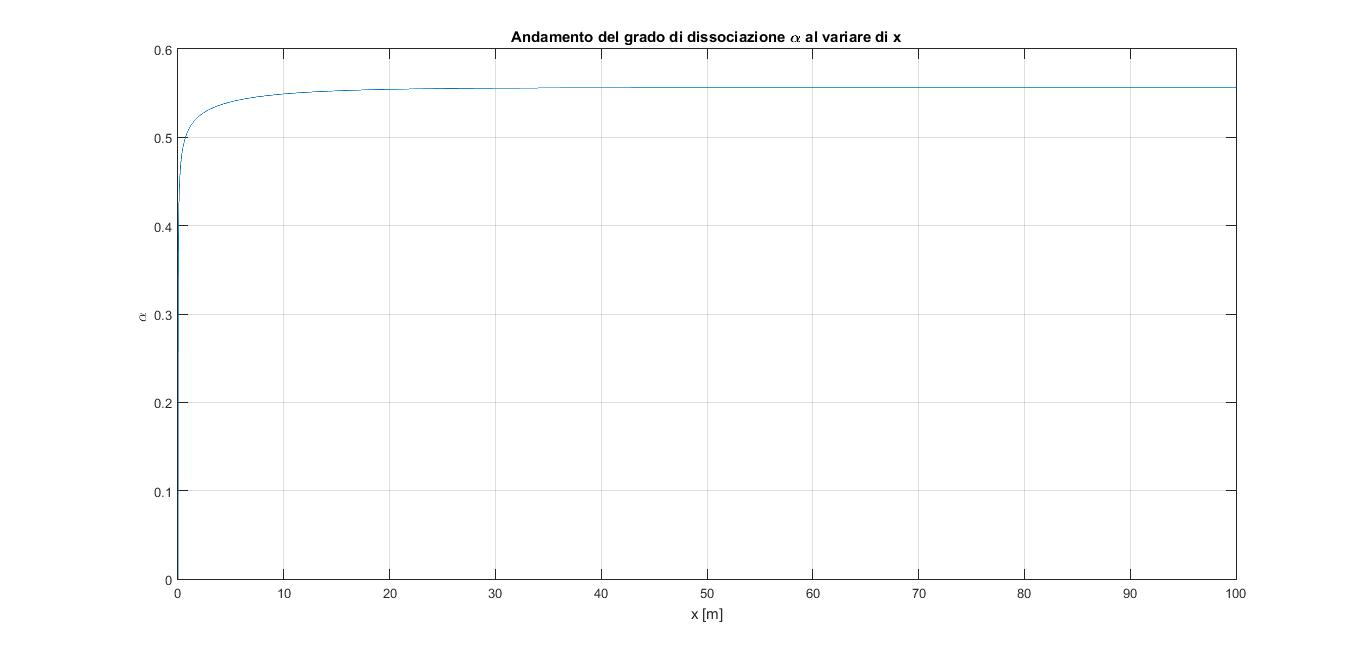
\includegraphics[width=150mm]{Immagini/alpha_rea}
		\caption{Andamento del grado di dissociazione in funzione dell'ascissa x, a valle dell'urto}
	\end{figure}
	\begin{figure}[htbp!]
		\centering
		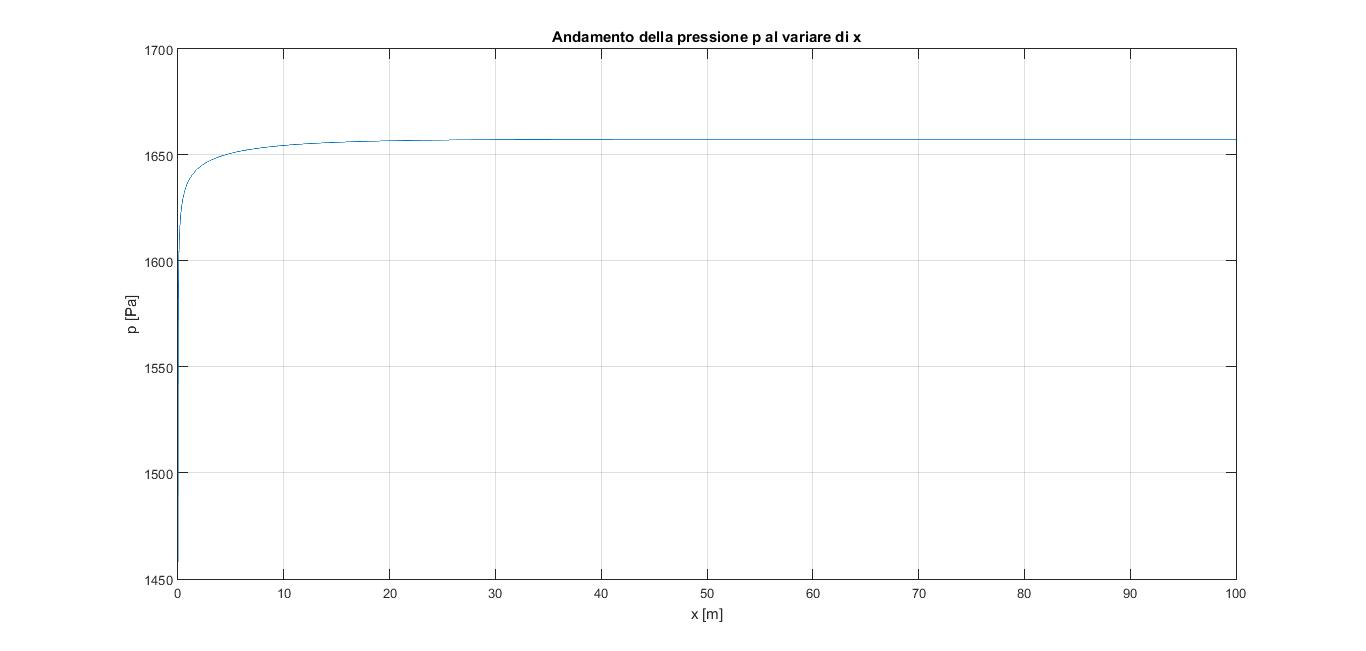
\includegraphics[width=150mm]{Immagini/p_rea}
		\caption{Andamento della pressione in funzione dell'ascissa x, a valle dell'urto }
	\end{figure}
	\newpage
	\begin{figure}[htbp!]
		\centering
		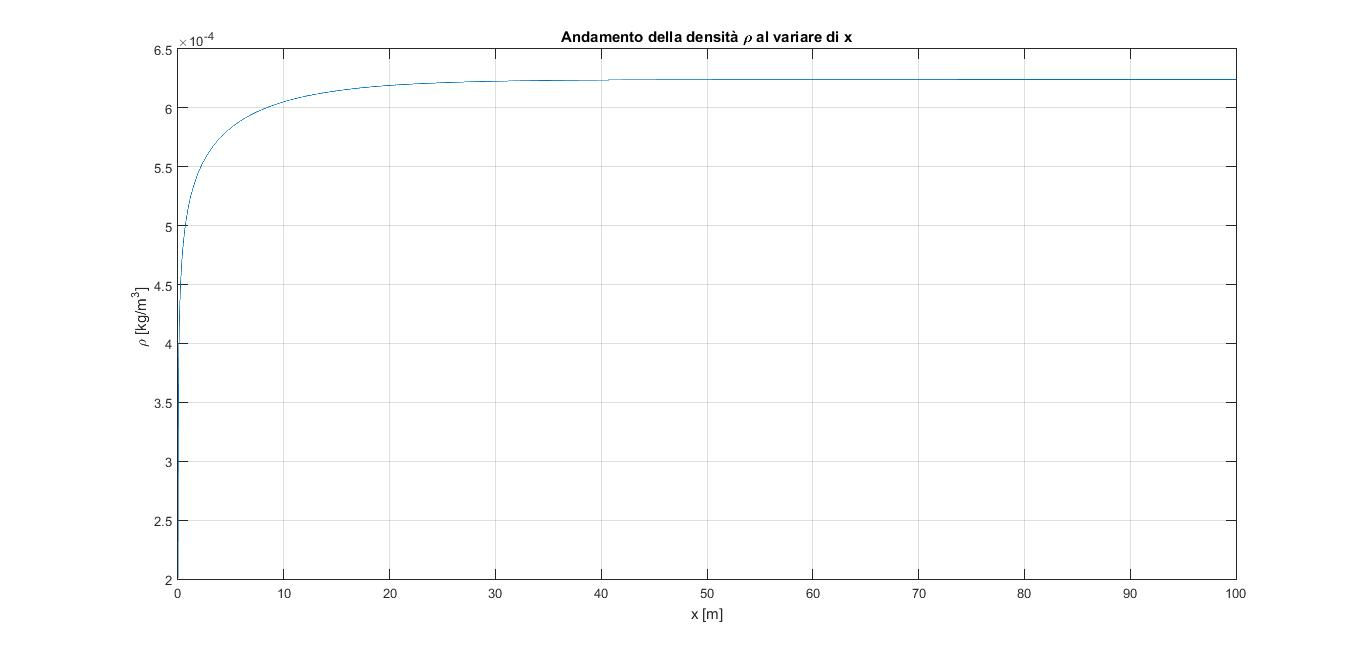
\includegraphics[width=150mm]{Immagini/rho_rea}
		\caption{Andamento della densit� in funzione dell'ascissa x, a valle dell'urto}
	\end{figure}
	\begin{figure}[htbp!]
		\centering
		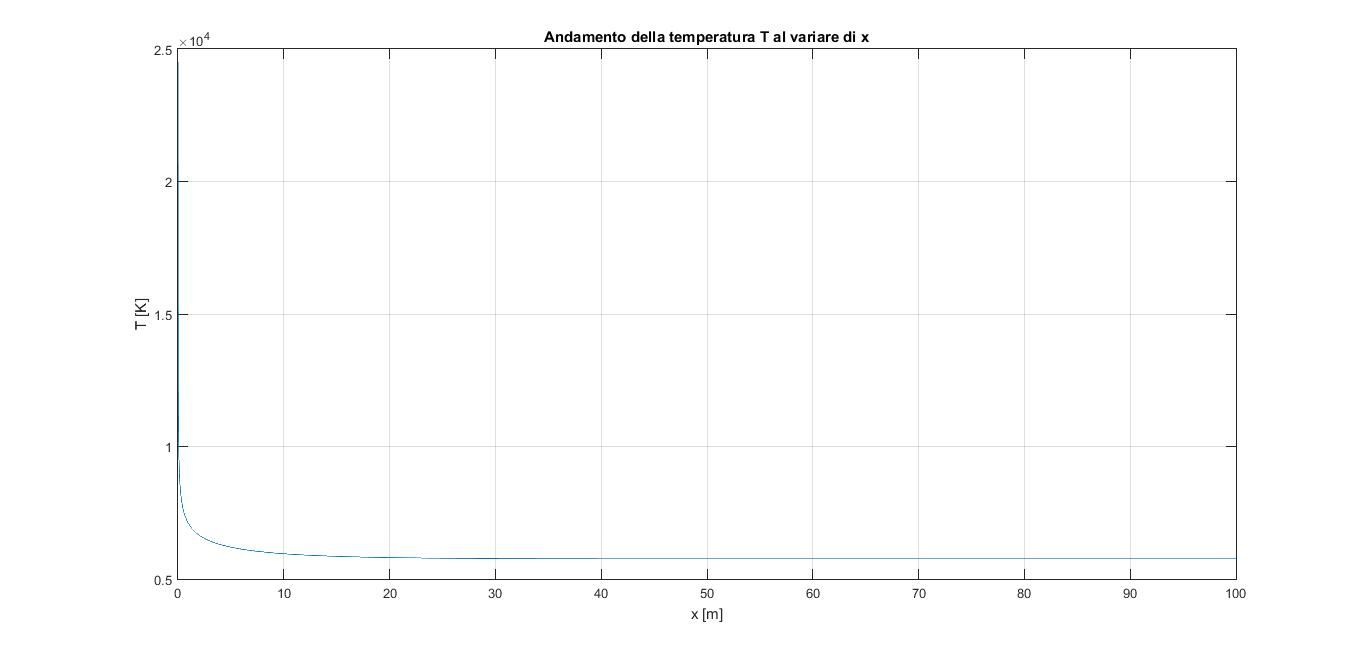
\includegraphics[width=150mm]{Immagini/T_rea}
		\caption{Andamento della temperatura in funzione dell'ascissa x, a valle dell'urto}
	\end{figure}
	\newpage
	\begin{figure}[htbp!]
		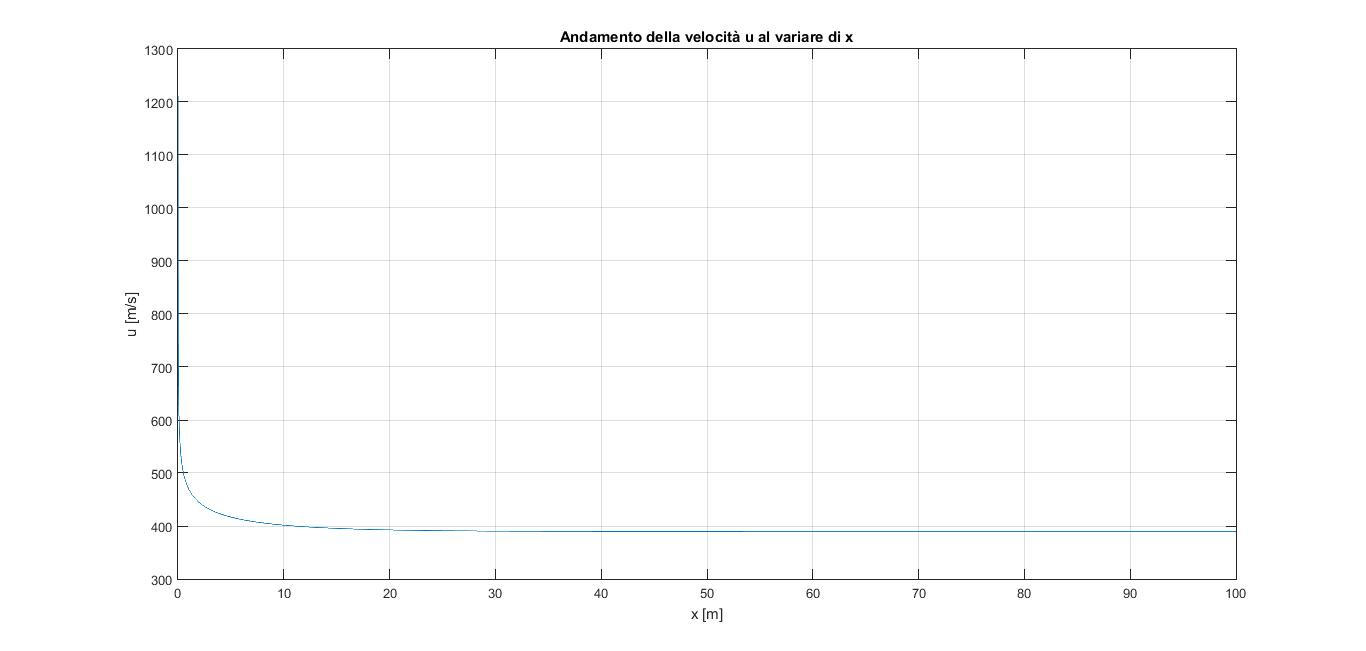
\includegraphics[width=150mm]{Immagini/u_rea}
		\caption{Andamento della velocit� in funzione dell'ascissa x, a valle dell'urto}
	\end{figure}


Immediatemente a valle dell'urto, l'azoto $N_{2}$ comincia a dissociare, per cui $\alpha $ aumenta; data l'alta temperatura iniziale $T_{2}$ , inizialmente il rateo di dissociazione � massimo.
Per la conservazione dell'energia, man mano la temperatura, e la velocit� diminuiscono, il grado di dissociazione $\alpha$ tende a stabilizzarsi verso una nuova condizione di equilibrio, dove l'azoto non riesce pi� a dissociare.\\
La diminuzione di temperatura ha effetto sul campo fluidodinamico, in particolare sulle $\rho$ ed
$u$ . La densit� aumenta rispetto al valore assunto immediatamente a valle dell'urto. E' noto che questo effetto si risente sullo spessore dello strato d'urto, che in alcuni casi pu� arrivare anche a dimezzarsi rispetto ad una situazione di flusso non reagente.\\
Inoltre nel caso considerato sappiamo che per la conservazione della portata, il prodotto $\rho u=cost $, per cui un'aumento della densit� comporta una dimunuzione della velocit� allo stesso modo.\\
Si osserva un aumento modesto  della pressione ($\approx 14\%$), questo sta ad indicare che a valle dell'urto si ha una ulteriore compressione.\\
\section{Flusso reagente in condotto divergente}
In questa sezione si vuole studiare il flusso di una miscela di gas formata da azoto parzialmente dissociata, in un condotto convergente-divergente.\\
Tuttavia nel nostro modello consideremo note le condizioni di flusso in gola occupandoci quindi di studiare l'evoluzione del flusso nel divergente. Da quanto detto precedentemente le condizioni in gola coincideranno con le condizioni iniziali del nostro problema. 
Il modello adottato � quello di flusso reagente (dissociazione/ricombinazione) non viscoso unidimensionale stazionario.Il divergente in cui si intende studiare il flusso � assunto di forma conica.\\
In questo caso il sistema di equazioni scritte per il caso precedente viene modificato con l'aggiunta del termine di variazione d'area $b_{1}=-\frac{\rho u}{A(x)}\frac{dA}{dx}$, dove $A(x)=\pi R^2(x)$ � l'andamento dell'area della sezione trasversale del condotto al variare di $x$ e $R(x)$ il raggio della sezione $x$.\\
Assumendo il condotto lungo $L=1$ $m$ e l'angolo di semiapertura $\beta$ pari a $5�$ si ha che $R(x)=0.03+tg(\beta)x$.
Il sistema di equazioni diventa:\\
$$\frac{dp}{dx}=\dot{p}=\frac{\left[ \frac{2(\alpha+1)}{3\alpha+7}\left(\frac{3}{4}\frac{R_{0}T}{PM_{N}}+\Delta h_{N}^0-\Delta h_{N_{2}}^0\right)-\frac{R_{0}T}{PM_{N2}}\right]\frac{\dot{W}}{u}-\frac{p}{\rho}\frac{b_{1}}{u}}{\frac{2(\alpha+1)}{3\alpha+7} +\frac{p}{\rho u^2}-1}$$
$$\frac{d\rho}{dx}=\frac{\dot{p}}{u^2}+\frac{b_{1}}{u^2}$$
$$\frac{du}{dx}=-\frac{\dot{p}}{\rho u}$$
$$\frac{dT}{dx}=\frac{2T}{p}\left( \frac{\alpha+1}{3\alpha+7}\right)\left[\dot{p}-\left(\frac{3}{4}\frac{R_{0}T}{PM_{N}}+\Delta h_{N}^0-\Delta h_{N_{2}}^0\right)\frac{\dot{W}}{u}\right]$$
$$\frac{d\alpha}{dx}=\frac{\dot{W}}{\rho u}$$\\\\

Supponendo di conoscere i valori di temperatura e pressione in gola, e supponendo che il gas sia in condizioni di equilibrio chimico in tale sezione si ha:\\
$\bullet$\quad $T_{g}=7000 K$\\
$\bullet$\quad $p_{g}=1.5 kPa$\\
$\bullet$\quad $\alpha_{g}=0.1434$\\
$\bullet$\quad $u_{g}=1900 m/s$\\

Il sistema di equazione viene implementato in ambiente Matlab.\\
Vengono riportati gli andamenti delle varie grandezze incognite, nonch� del numero di Mach, al variare dell'ascissa longitudinale x.\\

	\begin{figure}[htbp!]
		\centering
		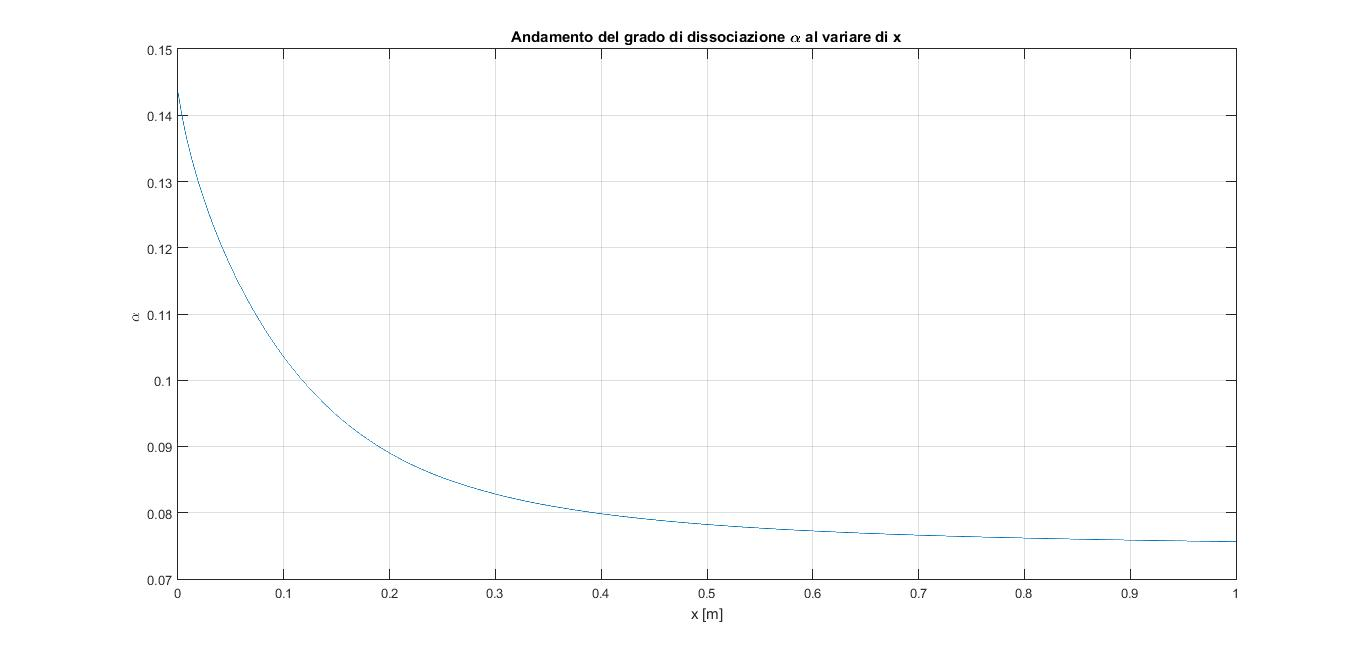
\includegraphics[width=150mm]{Immagini/alpha_div}
		\caption{Andamento del grado di dissociazione in funzione dell'ascissa x nel divergente}
	\end{figure}
	\begin{figure}[htbp!]
		\centering
		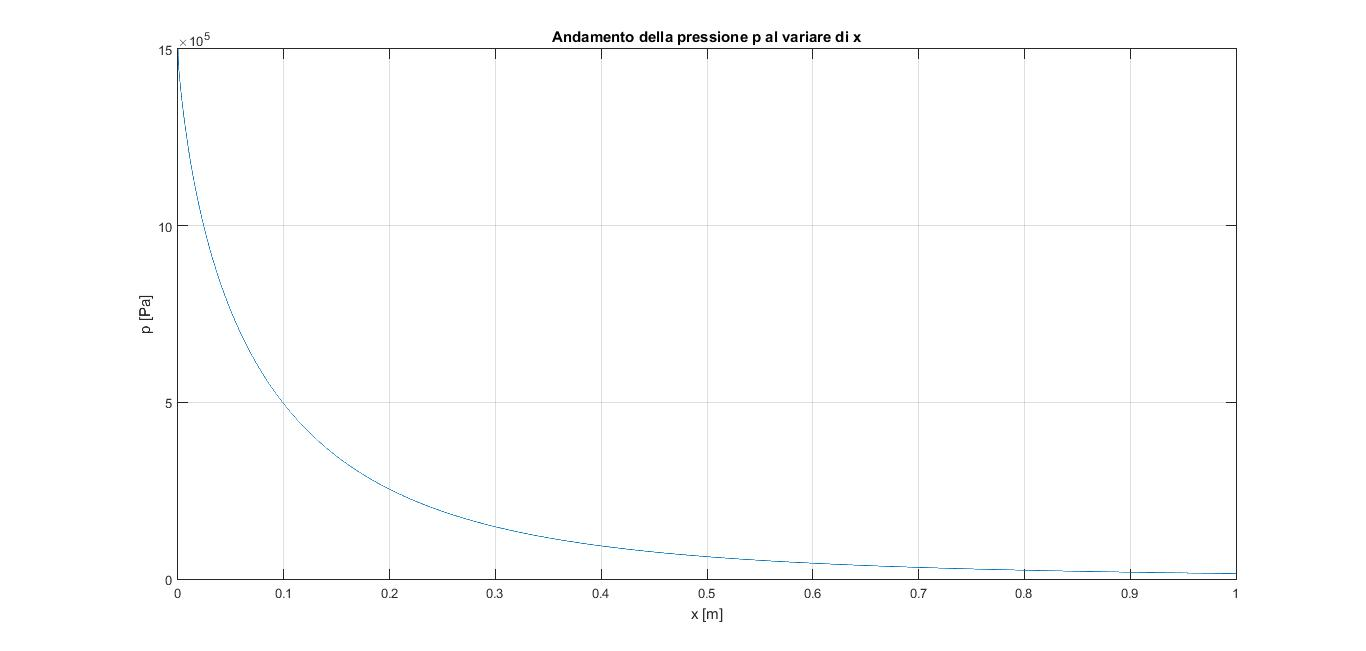
\includegraphics[width=150mm]{Immagini/p_div}
		\caption{Andamento della pressione in funzione dell'ascissa x nel divergente}
	\end{figure}
	\newpage
	\begin{figure}[htbp!]
		\centering
		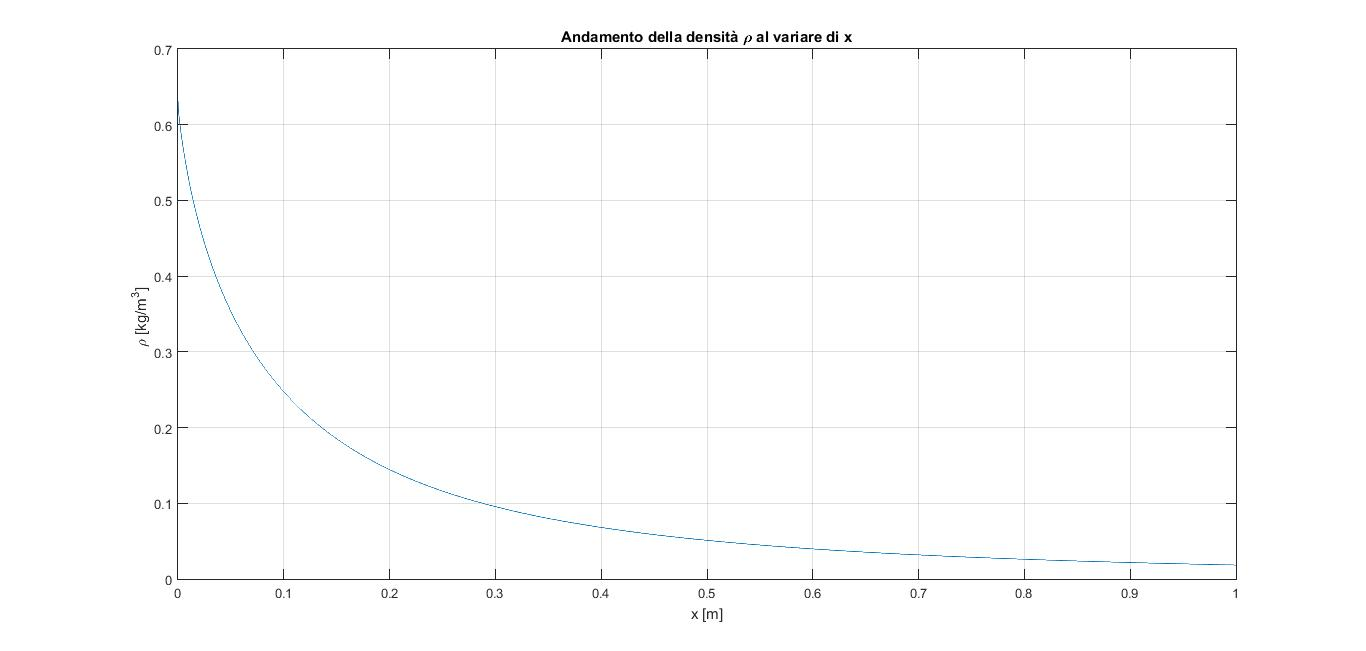
\includegraphics[width=150mm]{Immagini/rho_div}
		\caption{Andamento della densit� in funzione dell'ascissa x nel divergente}
	\end{figure}
	\begin{figure}[htbp!]
		\centering
		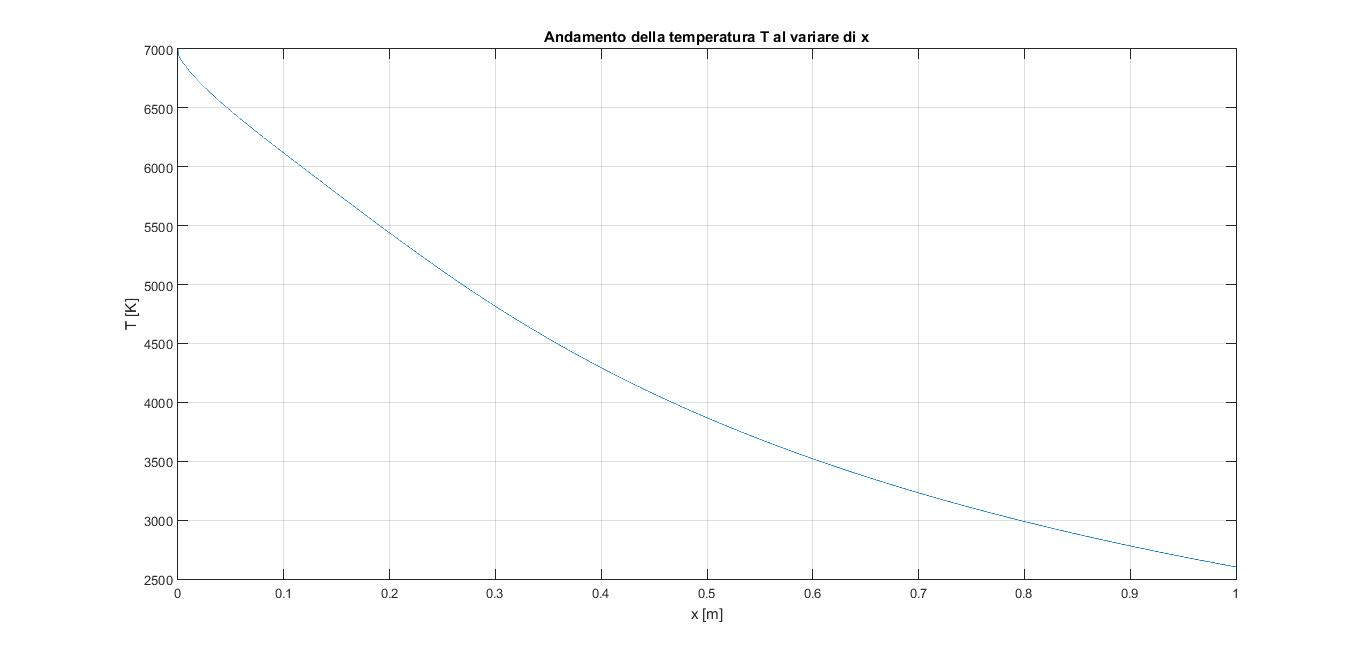
\includegraphics[width=150mm]{Immagini/T_div}
		\caption{Andamento della temperatura in funzione dell'ascissa x nel divergente}
	\end{figure}
	\begin{figure}[htbp!]
		\centering
		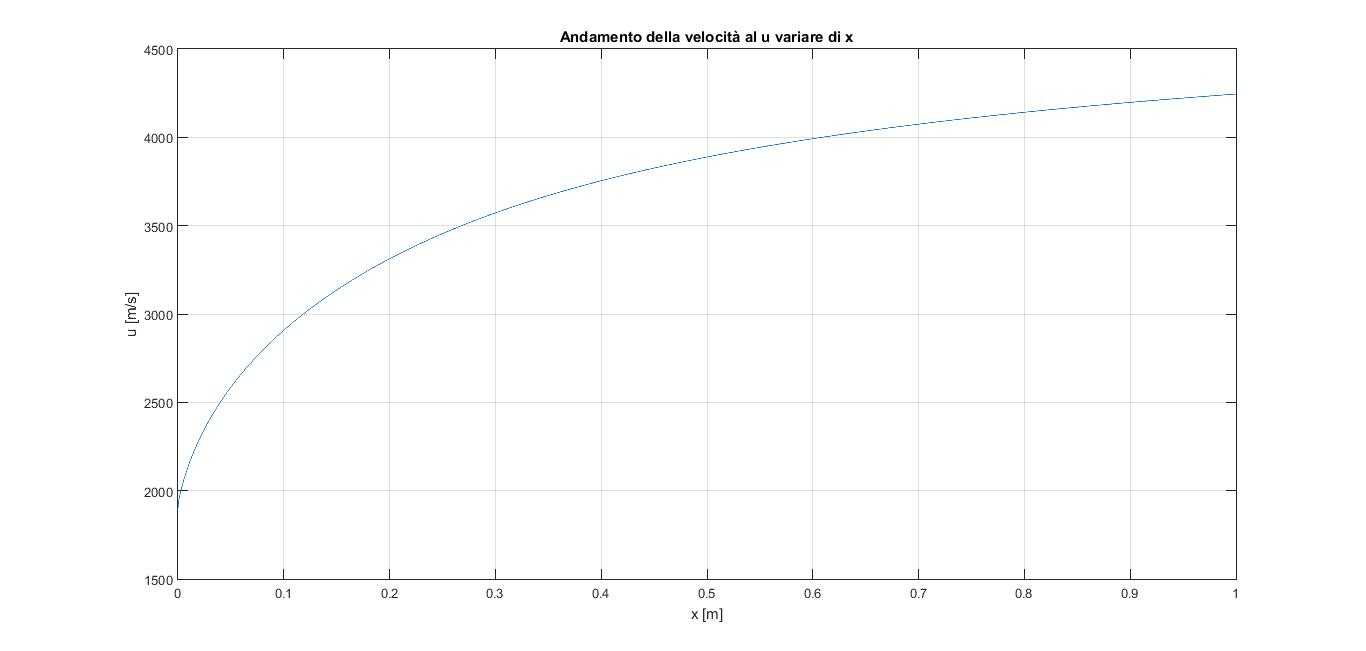
\includegraphics[width=150mm]{Immagini/u_div}
		\caption{Andamento della velocit� in funzione dell'ascissa x nel divergente}
	\end{figure}

Poich� il flusso � supersonico, il fluido subisce un'espansione nel divergente e quindi un calo della temperatura, come si nota dai grafici riportati in figura.\\
Il calo repentino di temperatura fa si che le costanti di velocit� di reazione $k_{f}$ e $k_{b}$ decrescano a loro volta; a questo punto i tempi di reazione diventano confrontabili con quelli chimici, e questo fa si che la reazione di ricombinazione dell'azoto non avvenga completamente. Si nota infatti come il grado di dissociazione dopo una brusca variazione iniziale si assesta su un valore prossimo a $0.075$ per il resto del condotto, si incorre cio� nel femonemo del congelamento. In sostanza il congelamento ha prodotto un intrappolamento di energia che non pu� essere riutilizzata.\\A causa del fenomeno del congelamento, ci si rende subito conto dell'impossibilit� di riprodurre le condizioni di volo di un velivolo ipersonico.  
Viene riportano in figura l'andamento del numero di Mach al variare l'ascissa longitudinale x.\\
\begin{figure}[htbp]
	\centering
	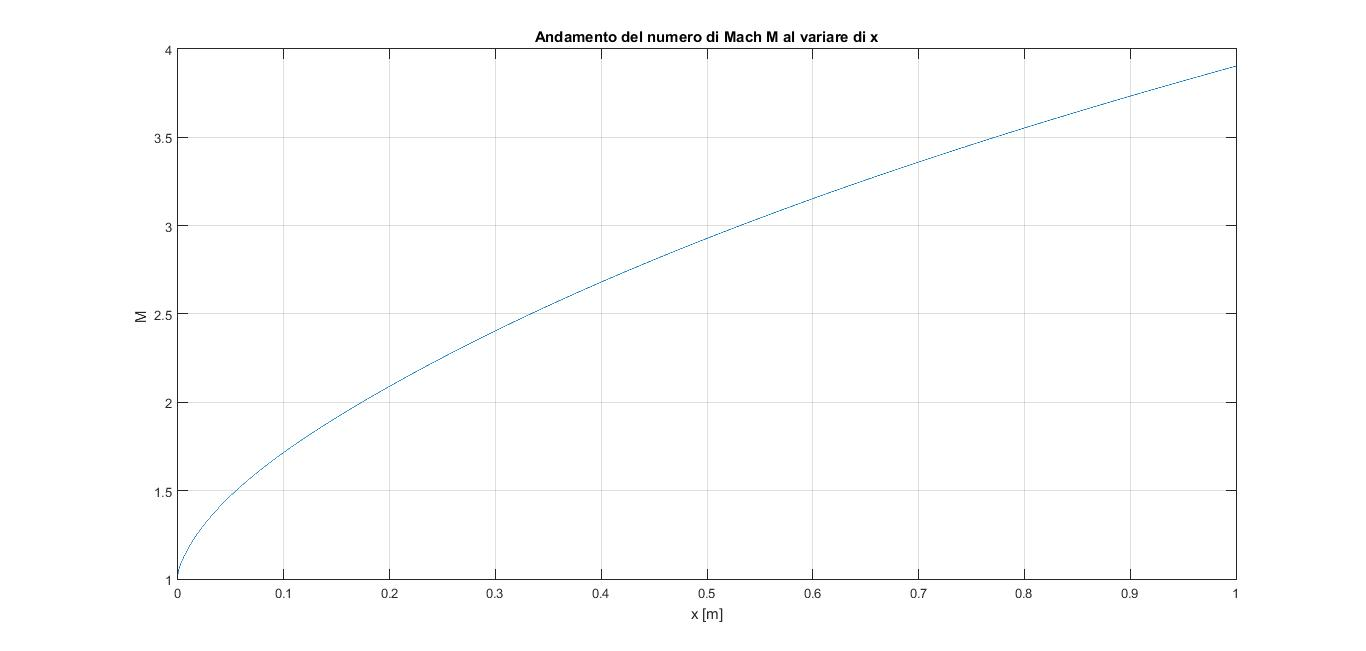
\includegraphics[width=150mm]{Immagini/mach_div}
	\caption{Andamento del numero di Mach in funzione dell'ascissa x nel divergente}
\end{figure}
  



    



\end{document}